\section{Dielectric-confined systems with charged slabs}\label{app::surfacecharge}

In this section, we will discuss the extension of the developed RBE algorithm to handle systems that involve both continuous surface charges and free ions. Without loss of generality, we assume two charged interfaces are located at $z=0$ and $z=H$ and with uniform surface charge density $\sigma_{\text{bot}}$ and $\sigma_{\text{top}}$. The system satisfies the charge neutrality condition \begin{equation}\label{eq::chargeneutrality}
    \sum_{i=1}^N q_i+(\sigma_{\text{bot}}+\sigma_{\text{top}})L_xL_y=0\;,
\end{equation}
so that the electrostatic energy and force of the system are both well-defined. When dealing with surface charges, it is common in the literature to handle discrete ions and continuous surface charges separately~\cite{spohr1997effect,yi2017note,yuan2021particle}. The former is typically treated as an infinite summation problem, while the latter is often obtained by solving an additional Poisson equation. %However, during the energy calculation, some divergent terms may arise. Since these terms do not affect the forces, they are often disregarded in a rough manner. 

In this manuscript, we employ a unified methodology where the continuous charge is treated as the limit distribution of an infinite set of discrete charges, following the framework outlined in Theorem~\ref{thm::FourDie}. To ensure accuracy, the parameters $M$ and $L_z$ are carefully selected to render both the ELC and remainder error terms negligible. As a result, we can accurately describe the force exerted on each mobile ion as:
\begin{equation}
\bm{F}^{\text{c}}(\bm{r}_i)=\bm{F}^{\text{c}}_{\text{real}}(\bm{r}_i)+\bm{F}^{\text{c}}_{\text{Fourier}}(\bm{r}_i)+\bm{F}^{\text{c}}_{\text{wall}}(\bm{r}_i),
\end{equation}
including the real space, the Fourier space, and ion-wall components. The real space component is given by
\begin{equation}\label{eq::F_real_detail}
\begin{split}
\bm{F}_{\text{real}}^{\te{c}}(\bm{r}_i)
& := -q_i\sum_{j=1}^{N} q_j \Biggg[\sum_{\bm{n}}{}^\prime \frac{\left(\bm{r}_{i,\bm{n}} - \bm{r}_{j}\right)}{\abs{\bm{r}_{i,\bm{n}} - \bm{r}_{j}}} K(\abs{\bm{r}_{i,\bm{n}} - \bm{r}_{j}}) \\
&+ \frac{1}{2} \sum_{\bm{n}} \sum_{l=1}^{M} \frac{\gamma_{l}^+\left(\bm{r}_{i,\bm{n}}-\bm{r}_{j+}^{(l)}\right)}{\left|\bm{r}_{i,\bm{n}}-\bm{r}_{j+}^{(l)}\right|} K\left(\left|\bm{r}_{i,\bm{n}}-\bm{r}_{j+}^{(l)}\right|\right)\\
&+\frac{1}{2}\sum_{\bm{n}}\sum_{l=1}^{M}\frac{\gamma_{l}^-\left(\bm{r}_{i,\bm{n}}-\bm{r}_{j-}^{(l)}\right)}{\left|\bm{r}_{i,\bm{n}}-\bm{r}_{j-}^{(l)}\right|}K\left(\left|\bm{r}_{i,\bm{n}}-\bm{r}_{j-}^{(l)}\right|\right)\Biggg]\\
&-\frac{q_i}{2}\sum_{j=1}^{N}q_j\sum_{\bm{n}}\sum_{l=1}^{M}\begin{pmatrix}
1&0&0\\
0&1&0\\
0&0&(-1)^l
\end{pmatrix}\Biggg[
\frac{\gamma_{l}^+\left(\bm{r}_{i,\bm{n}}-\bm{r}_{j+}^{(l)}\right)}{\left|\bm{r}_{i,\bm{n}}-\bm{r}_{j+}^{(l)}\right|}K\left(\left|\bm{r}_{i,\bm{n}}-\bm{r}_{j+}^{(l)}\right|\right)\\
&+\frac{\gamma_{l}^-\left(\bm{r}_{i,\bm{n}}-\bm{r}_{j-}^{(l)}\right)}{\left|\bm{r}_{i,\bm{n}}-\bm{r}_{j-}^{(l)}\right|}K\left(\left|\bm{r}_{i,\bm{n}}-\bm{r}_{j-}^{(l)}\right|\right)\Biggg]
\end{split}
\end{equation}
where $\bm{r}_{i,\bm{n}}=\bm{r}_{i}+\bm{\ell}$, and $K(r):=\text{erfc}(\alpha r)/r^2+2\alpha e^{-\alpha^2r^2}/(\sqrt{\pi}r)$. The Fourier component of force, $\bm{F}^{\text{c}}_{\text{Fourier}}$, has been provided in Eq.~\eqref{eq::52}. In practice, we use the RBE force $\bm{F}^{\text{c},*}_{\text{Fourier}}$ in Eq.~\eqref{eq::important} as an unbiased estimator to $\bm{F}^{\text{c}}_{\text{Fourier}}$, in which the formula of IBC term is more complicated than  {in} the case of  {a} neutral interface:
\begin{equation}\label{eq::IBC}
\begin{split}
\bm{F}_{\text{IBC}}^{M}(\bm{r}_i)=&-\frac{2\pi q_{i}}{L_xL_yL_z}\left[\mathcal{M}_{z}\left(1+\sum_{l=1}^{M}(-1)^{l}\left(\gamma_{+}^{(l)}+\gamma_{-}^{(l)}\right)\right)+\mathcal{M}_{z}^{M}\right]\V{\hat e_z}\\
&+\frac{2\pi q_i}{L_xL_yL_z}\sum_{j=1}^{N}q_j\left[z_i+\sum_{l=1}^{M}(-1)^{l}\left(\gamma_{+}^{(l)}z_{i+}^{(l)}+\gamma_{-}^{(l)}z_{i-}^{(l)}\right)\right]\V{\hat e_z}\\
&+\frac{2\pi q_iz_i}{L_xL_yL_z}\sum_{j=1}^{N}q_j\left[1+\sum_{l=1}^{M}\left(\gamma_{+}^{(l)}+\gamma_{-}^{(l)}\right)\right]\V{\hat e_z},
\end{split}
\end{equation}
where the $z$-direction dipole moments are defined via
\begin{equation}
\mathcal{M}_{z}:=\sum_{i=1}^{N}q_iz_i\quad\text{and}\quad \mathcal{M}_{z}^{M}:=\sum_{i=1}^{N}q_i\left[z_{j}+\sum_{l=1}^{M}\left(\gamma_{+}^{(l)}z_{j+}^{(l)}+\gamma_{-}^{(l)}z_{j-}^{(l)}\right)\right].
\end{equation}
It is important to highlight that if the free ions in the solution continue to fulfill condition Eq.~\eqref{eq:neutrality}, the last two terms in Eq.~\eqref{eq::IBC} vanish. 
The ion-wall component represents the force exerts on the mobile ions due to the charged walls, and is given by
\begin{equation}
\bm{F}_{\text{wall}}^{\te{c}}:=-2\pi z_{i}q_{i}\left[\sigma_{\text{top}}-\sigma_{\text{bot}}+\frac{(\sigma_{\text{top}}+\sigma_{\text{bot}})(\gamma_{\text{top}}-\gamma_{d})\left(1-\gamma_{\text{top}}^{\lceil M/2 \rceil}\gamma_{d}^{\lceil M/2 \rceil}\right)}{1-\gamma_{\text{top}}\gamma_{d}}\right]\V{\hat e_z}.
\end{equation}

% \section{High-performance implementation}\label{sec::ImpleStr}
% The RBE2D method is highly suitable for parallelization and vectorization. In this section, we present our implementation strategy for the RBE2D, incorporating MPI parallelization and Intel 512-bit SIMD (AVX-512 architecture) for vectorization. The latter enables simultaneous calculations of sixteen neighbors for single-precision floating-point operations (or eight for double precision). Intel One-API is employed for parallelization, encompassing MPI and AVX-512 instructions. The approach presented here is equally applicable to other parallelization models and vectorization instructions.

% Our implementation contributes in two main aspects. Firstly, we design communication operations that overlap with computations, reducing the overall serial portion. Secondly, we reformulate the expressions for the Fourier component and the dielectric correction component of the Coulomb interaction to reduce computational complexity. We discuss the techniques and insights as follows. Although these details may seem unrelated to the scientific aspects, we believe they are crucial for readers who are interested to reproduce or even improve upon our work.

% Due to the mini-batch strategy in the Fourier space, a serial importance sampling procedure and a global broadcast operation are required at each MD step. However, we mitigate this cost through the designed non-jammed communication, computation/communication overlapping, and parallel execution. Here are the details: assuming $\mathcal{M}$ MPI ranks are employed, $\mathcal{M}$ independent sampling processes are executed in parallel within each rank. The $1$st MPI rank broadcasts the samples to other ranks using a blocking operation. Concurrently, the computation step of the Coulomb interaction is executed while the samples in the $2$nd MPI rank are being broadcasted. This sequence is repeated $\mathcal{M}-1$ times, followed by a new sampling loop. This strategy evaluates and updates the samples every $\mathcal{M}$ steps, significantly reducing the sampling and global communication costs. It is crucial to emphasize that in order to generate independent samples, it is necessary for each rank to utilize a distinct initial random number seed.

% The image charge reflection, which accounts for dielectric jumps, is efficiently handled by precomputing the coefficients, as described in Section~\ref{sec::imagecharge}. This step, which incurs substantial computational resources in previous FFT-based methods~\cite{yuan2021particle}, involves lower additional costs in the RBE2D method developed in this paper.

% Furthermore, the speedup of the RBE2D is limited by the cost of the real-space calculation, specifically the computation of $F_i^{\text{real}}$. To enhance efficiency in the real space, the RBE2D implementation adopts the procedure from LAMMPS \cite{plimpton1995fast}, including domain decomposition, cell lists, communication design, and data structures. The directive-based offload technique \cite{brown2015optimizing} is employed for further acceleration. The computationally expensive error complementary function is efficiently computed using a combination of Taylor expansion, bit masking, and table look-up techniques, following the approach of LAMMPS.

% In many works that employ FFT-based methods as their electrostatic solvers, the real-space cutoff is balanced to ensure that the costs of the real and Fourier spaces are approximately equal. For the RBE2D, the real-space cutoff should be made smaller when accelerating calculations in the Fourier space. By combining other optimized techniques for real-space cutoffs with the RBE2D, even better acceleration can be achieved. Our ongoing project involves the combination of RBE2D with the random batch list algorithm \cite{liang2021random}, which is a recently developed acceleration technique for the real-space part.

\section{Simulation details}
The detailed parameters for simulations in Fig.~\ref{fig:den1} are listed in the following Table~\ref{Table::Dielec}.  {The log-log plots of the $W_2$ norm of difference on $\mathscr{P}(U)$ for simulations in Fig.~\ref{fig:3_1} and Figs.~\ref{fig:den1}(c-d) and~\ref{fig:den2} are shown in Figs.~\ref{fig:energy2d_3_1} and~\ref{fig:energy2d}, respectively.}
 {The time comparison between the RBE2D and PPPM methods are shown in Figs.~\ref{fig:timenondie} and~\ref{fig:timedie}, where the number of CPU cores is set to $64$ or $1024$ ($64$ cores per node) and the batch size is $P=200$.}

\renewcommand\arraystretch{1.7}
\begin{table}[h]
	\caption{The systems in Figure~\ref{fig:den1} are characterized by the following details, including the numbers of cations ($N_{\emph{cation}}$) and anions ($N_{\emph{anion}}$), the dimensions $L_x$, $L_y$, and $H$ (the slab height), the extended system length $L_z$, the surface charge densities ($\sigma_{u}$, $\sigma_{d}$), the factors of dielectric mismatch ($\gamma_{u}$ and $\gamma_{d}$) of the bottom and top walls, the diameter of ions $r_{\emph{d}}$, and the Bjerrum length ($\ell_{\emph{B}}$). The cutoff $r_c$ is set as $10\sigma$ and $4\sigma$ for producing (A-B) and (C-D), respectively.
}
	\centering
	\setlength{\tabcolsep}{0.6mm}{
		\begin{tabular}{|c|c|c|c|c|c|c|c|c|c|c|c|}
			\hline
			& $N_{\text{cation}}$ & $N_{\text{anion}}$ & $L_x$ [$\sigma$] & $L_y$ [$\sigma$] & $H$ [$\sigma$] & $\sigma_1 $ [$\frac{e}{\sigma^2}$] & $\sigma_2$ [$\frac{e}{\sigma^2}$] &$\gamma_{d}$ & $\gamma_{u}$ & $r_{\text{d}}$ [$\sigma$] & $\ell_{\text{B}}$ [$\sigma$] \\ \hline
      			%Fig.~\ref{fig:3_1} A-D& 750 & 2250 & 60  & 60 & 30   & -- & -- & -- & -- & 3.5 \\\hline
			%Fig.~\ref{fig:DiscreteLow} A-D & 0 & 486 & 90  & 90  & 30  & 0  & 0.06 & -- & -- &3.5    \\\hline
			%Fig.~\ref{fig:SurfaceCharge} A-D & 234 & 218 & 20  & 20  & 10 & -0.0008 & -0.0008 & -- & -- &0.7 \\\hline
			(A) &109  & 218  & 100 & 100 & 50 & -- & --  & 0.939  & 0.939  & 1 & 3.5 \\ \hline
			(B) &73  & 219 & 100 & 100 & 50 & --  & --  & 0.939  & 0.939  & 1 & 3.5 \\ \hline
			(C) & 23 & 42 & 42.9 & 42.9 & 8.4 & 0.01 & -0.02 & 0.6 & -0.33 & 2 & 2 \\ \hline
			(D) & 16 & 44 & 42.9 & 42.9 & 8.4 & 0.01 & -0.02  & 0.6 & -0.33 & 2 & 2 \\ \hline
	\end{tabular}}
	\label{Table::Dielec}
\end{table}

\begin{figure}[!ht]
\begin{center}
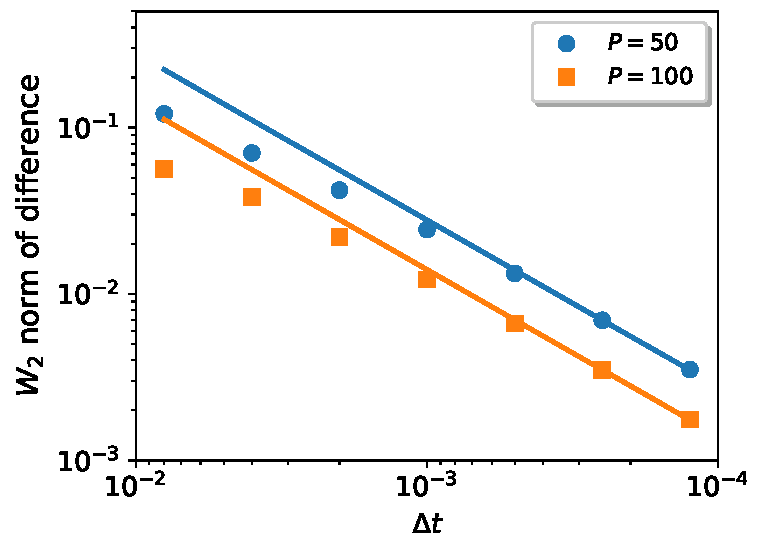
\includegraphics[width=0.6\textwidth]{figs/Energy_3_1.pdf}
\caption{ {The difference on the ensemble average of the total potential energy $\mathscr{P}(U)$ as a function of time step $\Delta t$ (unit: $\tau$). Data are shown for the same systems used in producing Figs.~\ref{fig:3_1} and $P=50$ and $100$. The solid lines indicate $O(\Delta t)$ scaling. The $W_2$ norm is used as the measurement.}}
\label{fig:energy2d_3_1}
\end{center} 
\end{figure}

\begin{figure}[htb]
\begin{center}
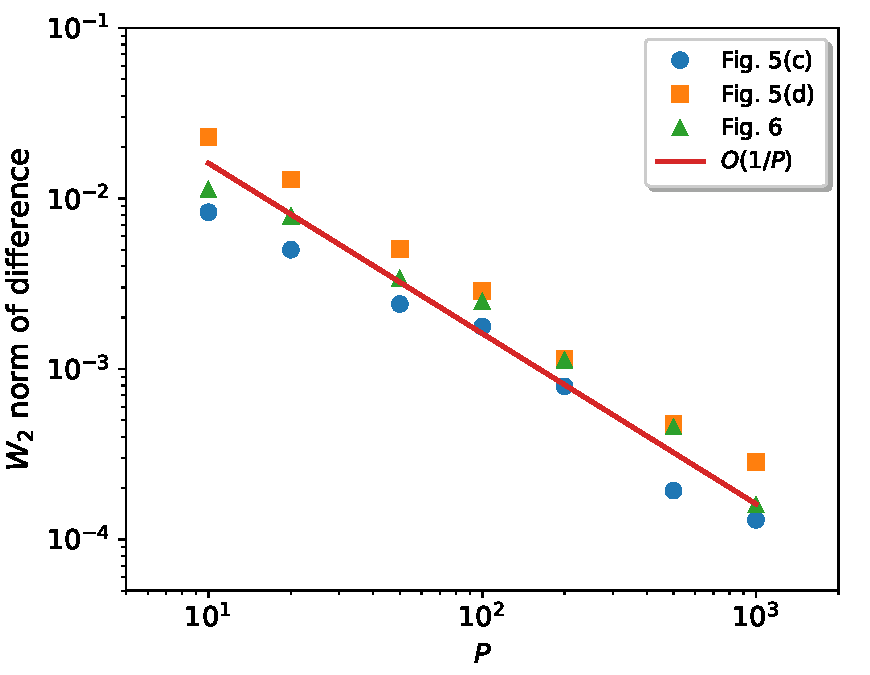
\includegraphics[width=0.6\textwidth]{figs/Energy.pdf}
\caption{The difference on the ensemble average of the total potential energy $\mathscr{P}(U)$ as a function of batch size $P$. Data are shown for the same systems used in producing Figs.~\ref{fig:den1}(c-d) and \ref{fig:den2}. The $W_2$ norm is used as the measurement.}
\label{fig:energy2d}
\end{center} 
\end{figure}

\begin{figure}[!ht]
\begin{center}
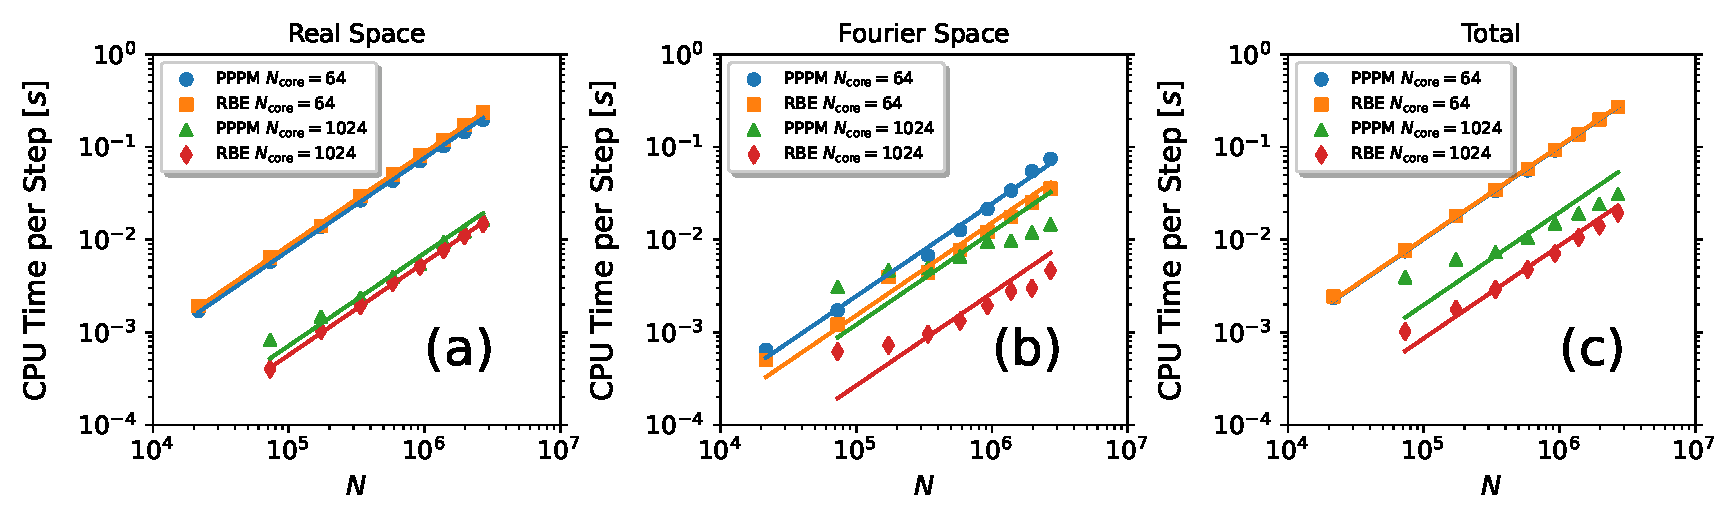
\includegraphics[width=1\textwidth]{figs/time_compare_nonsub.pdf}
\caption{CPU time comparison between the RBE2D and PPPM methods, with the number of CPU cores set to $64$ or $1024$ ($64$ cores per node) and a batch size of $P=200$. Data are shown for the same systems used in producing Fig.~\ref{fig:Time}(a), including CPU time per step of the real space component (Real), the Fourier space component (Fourier), and the total computation time (Total).
The results indicate that while the speedup achieved by the RBE2D method is minimal when the number of CPU cores is small ($N_{\mathrm{core}} = 64$), it becomes significantly more effective at reducing CPU time costs compared to the PPPM method when $N_{\mathrm{core}} = 1024$, primarily due to its lower communication overhead.
Note that in panel (c) the data points marked with blue circles are overlapped by those marked with orange squares.}
\label{fig:timenondie}
\end{center} 
\end{figure}

\begin{figure}[!ht]
\begin{center}
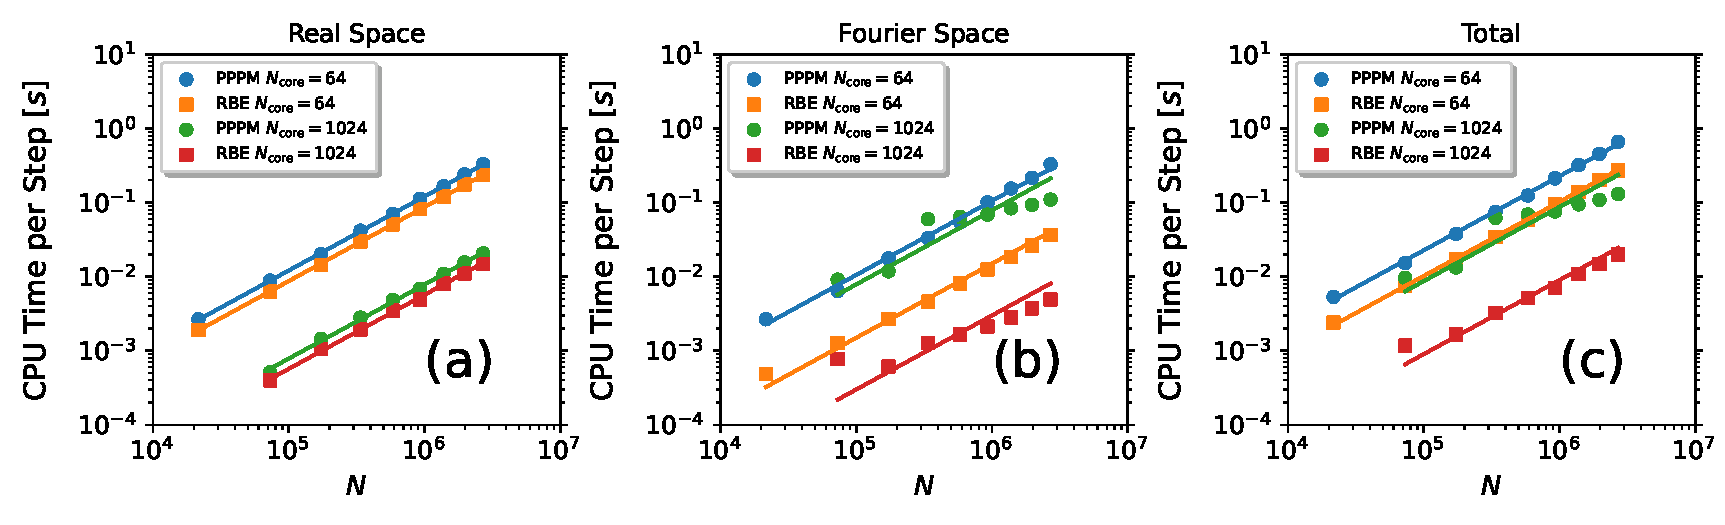
\includegraphics[width=1\textwidth]{figs/time_compare_withsub.pdf}
\caption{ {CPU time comparison between the RBE2D and ICM-PPPM methods, with the number of CPU cores set to $64$ or $1024$ ($64$ cores per node) and a batch size of $P=200$. Data are shown for the same systems as in Fig.~\ref{fig:Time}(a), but with a dielectric mismatch of $\gamma_{u} = \gamma_{d} = -0.9$. The CPU time per step is provided for the real space component (Real), Fourier space component (Fourier), and total computation time (Total).
Similarly, the results clearly show the speedup of the RBE2D method over the ICM-PPPM method, especially when the number of CPU cores is large.}}
\label{fig:timedie}
\end{center} 
\end{figure}